\documentclass[addpoints,spanish, 12pt,a4paper]{exam}
%\documentclass[answers, spanish, 12pt,a4paper]{exam}
  % \printanswers
\pointpoints{punto}{puntos}
\hpword{Puntos:}
\vpword{Puntos:}
\htword{Total}
\vtword{Total}
\hsword{Resultado:}
\hqword{Ejercicio:}
\vqword{Ejercicio:}

\usepackage[utf8]{inputenc}
\usepackage[spanish]{babel}
\usepackage{eurosym}
%\usepackage[spanish,es-lcroman, es-tabla, es-noshorthands]{babel}
\usepackage{pgf,tikz}
\usetikzlibrary{shapes, calc, shapes, arrows, math, babel}


\usepackage[margin=1in]{geometry}
\usepackage{amsmath,amssymb}
\usepackage{multicol}
\usepackage{yhmath}

\pointsinrightmargin % Para poner las puntuaciones a la derecha. Se puede cambiar. Si se comenta, sale a la izquierda.
\extrawidth{-2.4cm} %Un poquito más de margen por si ponemos textos largos.
\marginpointname{ \emph{\points}}

\usepackage{graphicx}

\graphicspath{{../img/}} 

\newcommand{\class}{4º Académicas}
\newcommand{\examdate}{\today}
\newcommand{\examnum}{Global 2ª evaluación}
\newcommand{\tipo}{A}


\newcommand{\timelimit}{50 minutos}

\renewcommand{\solutiontitle}{\noindent\textbf{Solución:}\enspace}


\pagestyle{head}
\firstpageheader{
\includegraphics[width=0.2\columnwidth]{header_left}}{\textbf{Departamento de Matemáticas\linebreak \class}\linebreak \examnum}{
\includegraphics[width=0.1\columnwidth]{header_right}}
\runningheader{\class}{\examnum}{Página \thepage\ of \numpages}
\runningheadrule

\DeclareUnicodeCharacter{2212}{-}
\begin{document}

\noindent
\begin{tabular*}{\textwidth}{l @{\extracolsep{\fill}} r @{\extracolsep{6pt}} }
\textbf{Nombre:} \makebox[3.5in]{\hrulefill} & \textbf{Fecha:}\makebox[1in]{\hrulefill} \\
 & \\
\textbf{Tiempo: \timelimit} & Tipo: \tipo 
\end{tabular*}
\rule[2ex]{\textwidth}{2pt}
Esta prueba tiene \numquestions\ ejercicios. La puntuación máxima es de \numpoints. 
La nota final de la prueba será la parte proporcional de la puntuación obtenida sobre la puntuación máxima. 

\begin{center}


\addpoints
 %\gradetable[h][questions]
	\pointtable[h][questions]
\end{center}

\noindent
\rule[2ex]{\textwidth}{2pt}

\begin{questions}


% \question[1] 
% \begin{solution} \end{solution}
% \addpoints

\question Resuelve por el método que consideres:
\begin{parts}
\part[1] 	$\left. \begin{gathered}
	  \frac{{3x}}{4} - \frac{{2y}}{3} = 1 \hfill \\
	  \frac{{5x}}{2} + \frac{{4y}}{3} = 14 \hfill \\ 
	\end{gathered}  \right\}$
\begin{solution} x=4; y=3 \end{solution}
% \part[1] $\left. \begin{gathered}
% 	  3x + 2y =  - 7 \hfill \\
% 	  \frac{1}{3}x - \frac{1}{4}y = \frac{1}{6} \hfill \\ 
% 	\end{gathered}  \right\}$
% \begin{solution} x=-1; y=-2 \end{solution} 
\end{parts}

% \question Resuelve mediante expresiones algebraicas:
% \begin{parts}
%     \part[1] Hace cinco años Pedro tenía triple edad que Jesús y dentro de un año sólo será el doble. ¿Cuáles son las edades de ambos en la actualidad?
% \begin{solution}$\left\{\begin{matrix}x-5=3(y-5) \\ x+1=2(y+1)\end{matrix}\right. \to  x = 23, \  y = 11 \to $ Pedro 23 años y Jesús 11 años \end{solution}
%     \part[1] Juan le dice a Luis: Actualmente mi edad es triple que la tuya, pero hace siete años era diez veces mayor que tú. ¿Qué edad tiene cada uno?

% \begin{solution} $\left\{\begin{matrix}x=3y \\ x-7=10(y-7)\end{matrix}\right. \to  x = 27, \  y = 9 \to$ Juan 27 años y Luis 9 años \end{solution}

% \end{parts}

% \question[1] Con dos clases de café de 5,4 euros/kg y 7,2 euros/kg se quiere obtener una mezcla cuyo precio resulte a 6 euros/kg. Calcula la cantidad que hay que poner de cada uno para lograr 600 kg de mezcla.

% \begin{solution} $\left\{\begin{matrix}5.4x+7.2y=6 \cdot 600 \\ x+y=600\end{matrix}\right. \to  x = 400.0, \  y = 200.0 \to$ 400 kg de 5,4 euros/kg y 200 kg de 7,2 euros/kg \end{solution}

\question[1] La cifra de las decenas de un número es triple que la de las unidades y el número disminuye en 36 cuando se invierte el orden de las cifras. Halla el número utilizando ecuaciones.
\begin{solution} $\left\{\begin{matrix}x=3y \\ 10x+y=10y+x+36\end{matrix}\right. \to  x = 6, \  y = 2 \to $ Número 62 \end{solution}

% \question Resuelve, justificadamente, los siguientes sistemas de inecuaciones:
% \begin{parts}
% \part[1] $\left\{\begin{matrix}\frac{x}{10-x}\geq 0 \\ x^2-9 >0\end{matrix}\right.$
% \begin{solution}  $\left(3, 10\right)$\end{solution}
% % \part[1] $\left\{\begin{matrix}4x+2y \geq 8 \\ -x+2y < 4  \\ -x < -2\end{matrix}\right.$
% % \begin{solution} \scalebox{.99}{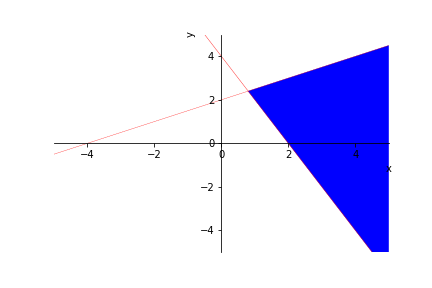
\includegraphics[width=1\columnwidth]{sistema_ine_ex0.png}}\end{solution}
% \end{parts}

% \question Resuelve la siguiente inecuación racional:\begin{parts} 
% \part[2] $\dfrac{x^{2} - 4}{x^{2} - 9} \geq  0$\begin{solution} $\left(-\infty, -3\right) \cup \left[-2, 2\right] \cup \left(3, \infty\right)$\end{solution} 
% \part[2] $\dfrac{x^{2} -4x +4}{x^{2} - 1} \geq  0$\begin{solution} $\left(-\infty, -1\right) \cup \left(1, \infty\right)$\end{solution} 
% \part[2] $\dfrac{x^{2} - 4}{x^{2} - 9} \leq  0$\begin{solution} $\left(-3, -2\right] \cup \left[2, 3\right)$\end{solution} 
% \part[2] $\dfrac{x^{2} -2x +1}{x^{2} - 9} \leq  0$\begin{solution} $\left(-3, 3\right)$\end{solution} 
% \end{parts} 


% \question Resuelve la siguiente inecuación con valor absoluto:\begin{parts} 
% \part[2] $| {2x - 4} | \leq  8$\begin{solution} $\left[-2, 6\right]$\end{solution} 
% \part[1] $| {2x + 3} | < 5$\begin{solution} $\left(-4, 1\right)$\end{solution} 
% \part[1] $| {3 - 2x} | \leq 7$\begin{solution} $\left[-2, 5\right]$\end{solution} 
% \part[1] $| {6 - 8x} | \geq 10$ \begin{solution} $\left(-\infty, - \frac{1}{2}\right] \cup \left[2, \infty\right)$ \end{solution} 
% \end{parts} 


% \question Resuelve el siguiente sistema de inecuaciones con dos incógnitas (puedes usar el plano cartesiano que se adjunta):

% \begin{parts} 
% \part[2] $\left\{\begin{matrix}4x+2y \geq 8 \\ -x+2y < 4\end{matrix}\right.$\begin{solution}  \scalebox{.99}{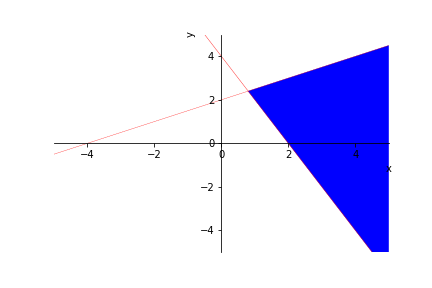
\includegraphics[width=1\columnwidth]{sistema_ine_ex0.png}}\end{solution}

% \part[2] $\left\{\begin{matrix}2x+y \leq 4 \\ 2x-y > 2 \\ y>-2 \\ x>0\end{matrix}\right.$\begin{solution}  \scalebox{.99}{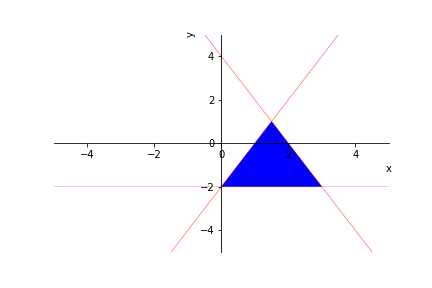
\includegraphics[width=1\columnwidth]{sistema_ine_ex1.png}}\end{solution} 
% \end{parts} 


\question Calcular el dominio de las siguientes funciones:
\begin{parts} 
% \part[1] $f(x)=\dfrac{2x+1}{x^{2} - 4 x + 3}$\begin{solution} $\left(-\infty, 1\right) \cup \left(1, 3\right) \cup \left(3, \infty\right)$\end{solution} 
% \part[1] $f(x)=\sqrt{x^2+3x+2}$\begin{solution} $\left(-\infty, -2\right] \cup \left[-1, \infty\right)$\end{solution} 
\part[1] $f(x)=\dfrac{2x-1}{x^{2} + 4 x + 3}$\begin{solution} $\left(-\infty, -3\right) \cup \left(-3, -1\right) \cup \left(-1, \infty\right)$\end{solution} 
\part[1] $f(x)=\sqrt{x^{2} - 3 x + 2}$\begin{solution} $\left(-\infty, 1\right] \cup \left[2, \infty\right)$\end{solution} 
% \part[1] $f(x)=\dfrac{1}{2-\sqrt{x}}$\begin{solution} $\left[0, 4\right) \cup \left(4, \infty\right)$\end{solution} 

% Examen alumno después
% \part[1] $f(x)=\sqrt{\dfrac{x^2-9}{1-x}}$\begin{solution} $\left(-\infty, -3\right] \cup \left(1, 3\right]$\end{solution} 
% \part[1] $f(x)=x^4-13x^2+36$\begin{solution} $\mathbb{R}$\end{solution}

\end{parts} 


% \question Dada la función: $$y=\begin{cases} 3 - 2 x & \text{si}\: x < -1 \\3 & \text{si}\: -1\leq x \leq 3 \\x + 3 & \text{si}\: x>3 \end{cases}$$
% \begin{parts}
% \part[2] Representa la función (puedes usar el plano cartesiano que se adjunta)
% \begin{solution} \scalebox{.6}{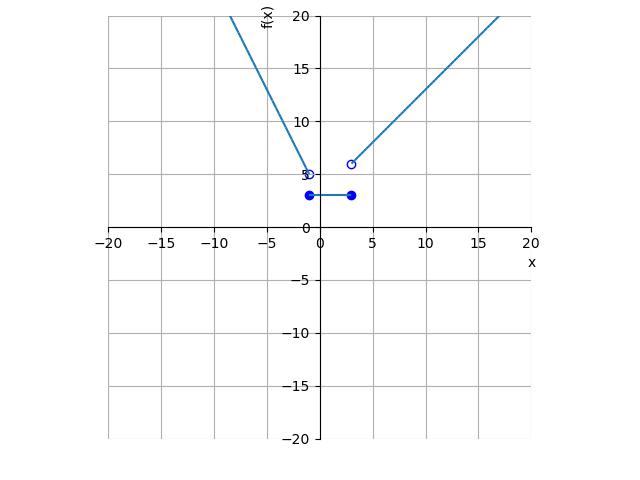
\includegraphics[width=1\columnwidth]{ex_funcion_a_trozos_5}}\end{solution}\part[1] Indica: \begin{itemize}
%     \item Dominio y Recorrido
%     \item Intervalos de crecimiento y decrecimiento
%     \item Máximos y mínimos relativos
%     \item Discontinuidades
% \end{itemize}
% \end{parts}

% \question Dada la función: $$y=\begin{cases} 2 x + 3 & \text{si}\: x < -2 \\3 & \text{si}\: -2\leq x \leq 2 \\3 - x & \text{si}\: x > 2 \end{cases}$$
% \begin{parts}
% \part[2] Representa la función (puedes usar el plano cartesiano que se adjunta)
% \begin{solution} \scalebox{.6}{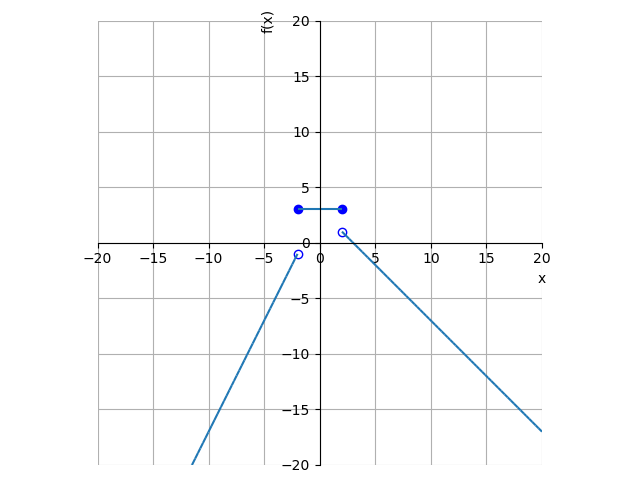
\includegraphics[width=1\columnwidth]{ex_funcion_a_trozos_4}}\end{solution}\part[1] Indica: \begin{itemize}
%     \item Dominio y Recorrido
%     \item Intervalos de crecimiento y decrecimiento
%     \item Máximos y mínimos relativos
%     \item Discontinuidades
% \end{itemize}
% \end{parts}


% \question Dada la función: $$y=\begin{cases} 3 - 2 x & \text{si}\: x < 1 \\- x^{2} + 6 x - 8 & \text{si}\: x \geq 1 \end{cases}$$
% \begin{parts}
% \part[2] Representa la función (puedes usar el plano cartesiano que se adjunta)
% \begin{solution} \scalebox{.6}{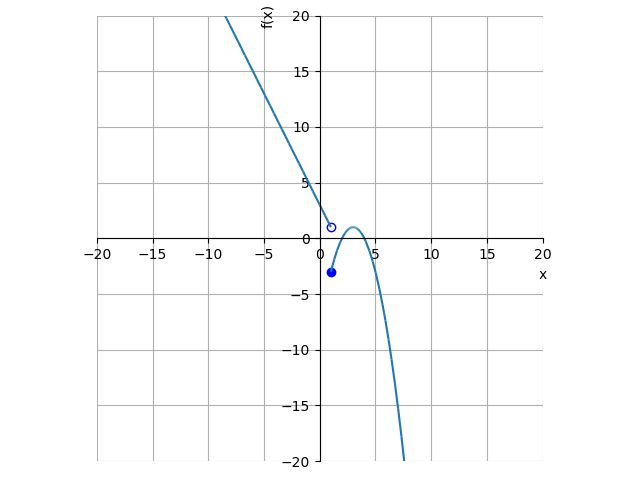
\includegraphics[width=1\columnwidth]{ex_funcion_a_trozos_3}}\end{solution}\part[1] Indica: \begin{itemize}
%     \item Dominio y Recorrido
%     \item Intervalos de crecimiento y decrecimiento
%     \item Máximos y mínimos relativos
%     \item Discontinuidades
% \end{itemize}
% \end{parts}

% \question Dada la función: $$y=\begin{cases} 2 x - 3 & \text{si}\: x < -1 \\- x^{2} + 2 x & \text{si}\: x\geq -1 \end{cases}$$
% \begin{parts}
% \part[2] Representa la función (puedes usar el plano cartesiano que se adjunta)
% \begin{solution} \scalebox{.6}{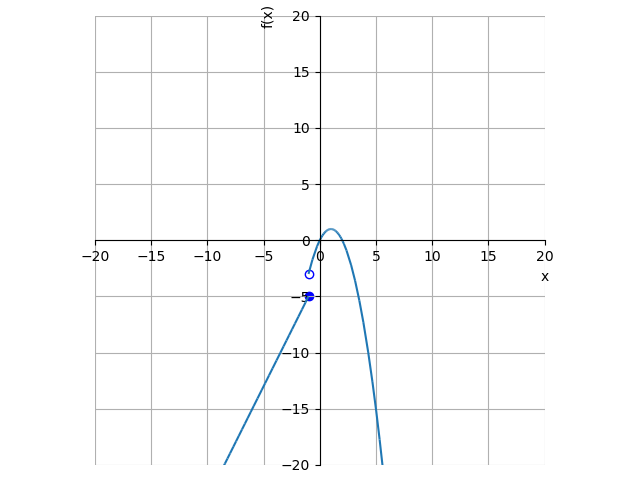
\includegraphics[width=1\columnwidth]{ex_funcion_a_trozos_2}}\end{solution}\part[1] Indica: \begin{itemize}
%     \item Dominio y Recorrido
%     \item Intervalos de crecimiento y decrecimiento
%     \item Máximos y mínimos relativos
%     \item Discontinuidades
% \end{itemize}
% \end{parts}

% \question Dada la función: $$y=\begin{cases} 2 x + 2 & \text{si}\: x \leq -1 \\x^{2} - 2 x &  \text{si} \: x > -1 \end{cases}$$
% \begin{parts}
% \part[2] Representa la función (puedes usar el plano cartesiano que se adjunta)
% \begin{solution} \scalebox{.6}{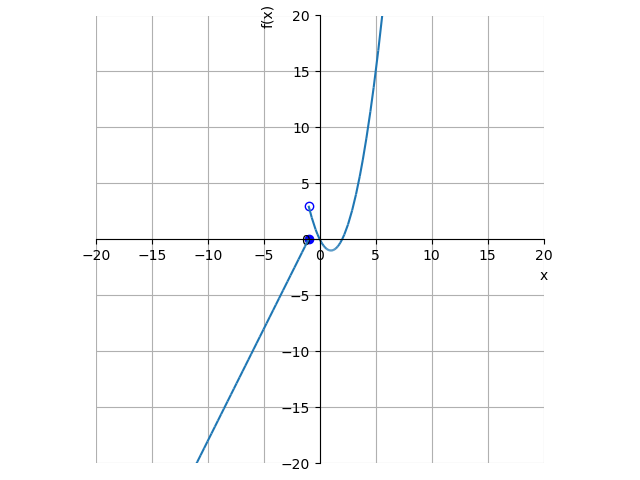
\includegraphics[width=1\columnwidth]{ex_funcion_a_trozos_0}}\end{solution}
% \part[1] Indica: \begin{itemize}
%     \item Dominio y Recorrido
%     \item Intervalos de crecimiento y decrecimiento
%     \item Máximos y mínimos relativos
%     \item Discontinuidades
% \end{itemize}
% \end{parts}

\question Dada la función: $$y=\begin{cases} 3 - 2 x & \text{si}\: x < 1 \\x^{2} - 6 x + 8 & \text{si}\: x\geq 1 \end{cases}$$
\begin{parts}
\part[2] Representa la función (puedes usar el plano cartesiano que se adjunta)
\begin{solution} \scalebox{.6}{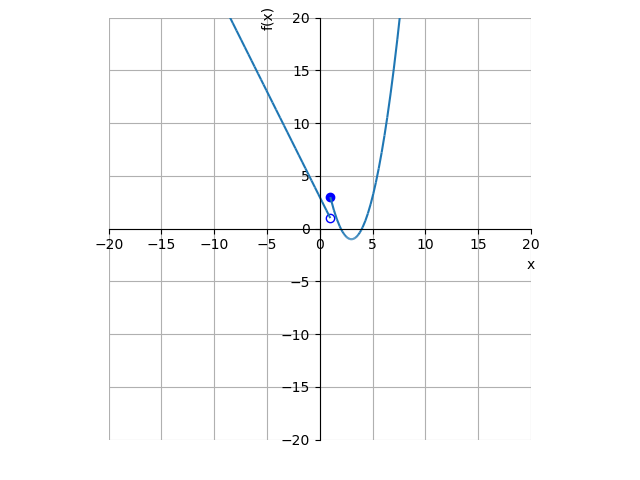
\includegraphics[width=1\columnwidth]{ex_funcion_a_trozos_1}}\end{solution}
\part[1] Indica: \begin{itemize}
    \item Dominio y Recorrido
    \item Intervalos de crecimiento y decrecimiento
    \item Máximos y mínimos relativos
    \item Discontinuidades
\end{itemize}
\end{parts}

% \question Dada la función: $$f(x)=\begin{cases} 2 x - 4 & \text{si}\: x < -2 \\- x^{2} + 4 x - 3 & \text{si}\: -2 \leq x < 3 \\3 & \text{si}\: x > 3 \end{cases}$$
% \begin{parts}
% \part[2] Representa la función (puedes usar el plano cartesiano que se adjunta)
% \begin{solution} \scalebox{.6}{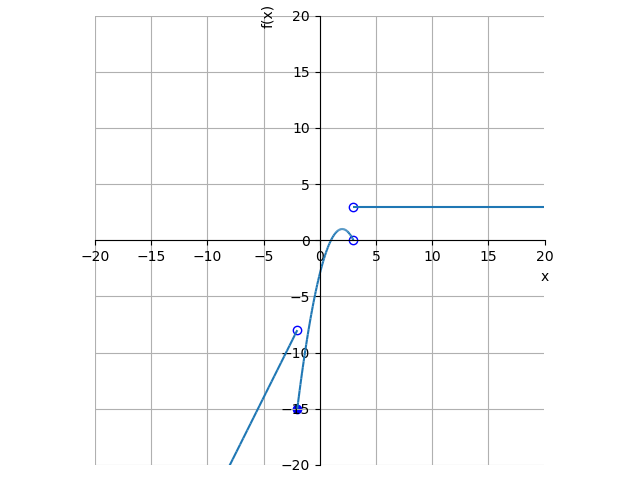
\includegraphics[width=1\columnwidth]{ex_funcion_a_trozos_6}}\end{solution}
% \part[1] Indica: \begin{itemize}
%     \item Dominio y Recorrido
%     \item Intervalos de crecimiento y decrecimiento
%     \item Máximos y mínimos relativos
%     \item Discontinuidades
% \end{itemize}
% \end{parts}

\question[2] La altura, h, a la que se encuentra en cada instante, t, una piedra que lanzamos hacia arriba con una velocidad de 20 m/s es $h = 16t— 2t^2$. 
\begin{parts}
    \part Representa gráficamente la función y di cuál es su dominio de definición. 
    \part ¿En qué momento alcanza su altura máxima? ¿Cuál es esa altura?
    \part ¿En qué momento llega la piedra al suelo? 
    \part ¿En qué intervalo de tiempo la piedra está a una altura superior a 14 metros?
\end{parts} 

% \question[2] La altura, h, a la que se encuentra en cada instante, t, una pelota que lanzamos hacia arriba con una velocidad de 25 m/s es $h = 8t— t^2$. 
% \begin{parts}
%     \part Representa gráficamente la función y di cuál es su dominio de definición. 
%     \part ¿En qué momento alcanza su altura máxima? ¿Cuál es esa altura?
%     \part ¿En qué momento llega la pelota al suelo? 
%     \part ¿En qué intervalo de tiempo la pelota está a una altura superior a 7 metros?
% \end{parts} 


% \question Un cuerpo, en caída libre, adquiere una velocidad que aumenta unos 35 km/h cada segundo. Dejamos caer una bola de hierro desde lo alto de un acantilado.
% \begin{parts}
% \part Escribe la expresión analítica de la función que relaciona el tiempo desde que se dejó caer con la velocidad a la que cae
% \part Represéntala en unos ejes.
% \part Suponiendo que la bola no se frena con el aire, ¿qué velocidad llevará a los 3 s? ¿Y a los 10 s?
% \part Si la bola choca contra el suelo a una velocidad de 420 km/h, ¿cuánto ha tardado en caer?    
% \end{parts}  

% \question Las ventas obtenidas por una empresa han sido de $28000$ \euro \ con unos gastos
% en publicidad de $3000$ \euro \ y de 39 000 \euro \ con unos gastos publicitarios de
% $5 000$ \euro.
% Si las ventas siguen una función lineal, obtén la expresión analítica de esa función y estima cuáles serán las ventas si se invierte en publicidad $4 000$ \euro.
% \begin{solution}
%     y = 28 000 + 5,5(x – 3 000)
% y (4 000) = 33 500 euros
% \end{solution}

% \question El precio del billete de una línea de cercanías depende de los kilómetros recorridos. Por 57 km he pagado $2.85$ euros, y por 168 km, $13.4$ euros. Si el precio sigue una función lineal, obtén la expresión analítica de esa función y calcula el precio de un billete para una distancia de 100 km.
% \begin{solution}
%     y = 2,85 + 0,095(x – 57)
% y (100) = 6,94 euros
% \end{solution}

\question Dada la función $f(x)=\left|2x+4\right|$
\begin{parts} 
\part[2] Transforma la función a una función a trozos equivalente
\begin{solution} $f(x) =
\left\{
	\begin{array}{clc}
		-(2x +4)   & \mbox{si } & x < -2 \\
		2x +4   & \mbox{si } & x \geq -2
	\end{array}
\right.$
\end{solution}
% \part[2] Representa la función gráficamente 
% \begin{solution} 

% \begin{tikzpicture}[domain=-4.1:3.1 ,>=triangle 45, scale=0.35]

% \tikzmath{
% 			\a = 1; \b = -2; \c = 1; 
% 			\v = - \b / ( 2 * \a);
% 			\m1 = -2; \n1 = -4;
% 			\m3 = 2; \n3 = 4;
% 			\xmin1 = - 4.1; \xmax1 = -2;
% 			\xmin2 = - 2; \xmax2 = -2;
% 			\xmin3 = -2; \xmax3 = 3.1;
%           }
          
 
% \draw[color=red, domain=\xmin1 -0.5:\xmax1]    plot (\x,{\m1*(\x) + \n1}) node[right] {};

% %\draw [red] (\xmax1,{\m1*(\xmax1) + \n1}) circle (0.25) node [left] {};

% %\draw[color=red, domain=\xmin2:\xmax2]    plot (\x,{\a*(\x)^2 + \b *\x + \c})             node[right] {}; 
% %\draw [red, fill] (\xmin2,{\a*(\xmin2)^2 + \b *\xmin2 + \c}) circle (0.25) node [left] {};
% %\draw [red] (\xmax2,{\a*(\xmax2)^2 + \b *\xmax2 + \c}) circle (0.25) node [left] {};

% \draw[color=red, domain=\xmin3  :\xmax3 + 0.1]    plot (\x,{\m3*(\x) + \n3}) node[right] {};
% %\draw [red] (\xmin3,{\m3*(\xmin3) + \n3}) circle (0.25) node [left] {};

% \draw[very thin,color=lightgray,dash pattern=on 1pt off 1pt] (\xmin1 - 0.5, \a * \v * \v + \b * \v + \c - 0.5) grid (\xmax3 + 0.5 , \a * \xmin2 * \xmin2 + \b * \xmin2 + \c + 0.5);

% \draw[<->] (\xmin1 -1,0) -- (\xmax3 + 1,0) node[right] {$x$};
% \draw[<->] (0,\a * \v * \v + \b * \v + \c - 0.5) -- (0, \a * \xmin2 * \xmin2 + \b * \xmin2 + \c + 0.5 ) node[above] {$y$};

% \end{tikzpicture}  
% \end{solution}
% \part[1] Indica el \emph{dominio} y el \emph{recorrido} de la función utilizando la notación de conjuntos de números reales
% \begin{solution} $Dom(f)=\mathbb{R} $ \\
% $ Im(f)=\left[0, +\infty\right]$
% \end{solution}
\end{parts}

% \question[1] Responde a las siguientes cuestiones:
% \begin{parts}
% \part Indica la ecuación o la expresión analítica correspondiente a una recta que pasa por el punto de coordenadas $\left(0,1\right)$ y cuya pendiente vale 3
% \begin{solution}
% $y=3x+1$
% \end{solution}
% \part Razona, sin representar ni calcular puntos de la gráfica, el número de puntos de corte de la función $y=(x-1)^2+1$ con el eje $OX$ 
% \begin{solution}
% Ninguno, porque $y\geq 1 \ \forall x$
% \end{solution}
% \end{parts}

% \question[1] Responde y justifica las siguientes cuestiones:
% \begin{parts}
% \part ¿Existe alguna función lineal que solo corte al eje $OX$ por $\left(3,0\right)$ y no al eje $OY$? En caso afirmativo da la ecuación de dicha función.  
% \part ¿Existe alguna función lineal que solo corte al eje $OY$ por $\left(0,3\right)$ y no al eje $OX$? En caso afirmativo da la ecuación de dicha función.

% \end{parts}\question[1] Responde a las siguientes cuestiones:
% \begin{parts}
% \part Indica la ecuación o la expresión analítica correspondiente a una recta que pasa por el punto de coordenadas $\left(0,1\right)$ y cuya pendiente vale 3
% \begin{solution}
% $y=3x+1$
% \end{solution}
% \part Razona, sin representar ni calcular puntos de la gráfica, el número de puntos de corte de la función $y=(x-1)^2+1$ con el eje $OX$ 
% \begin{solution}
% Ninguno, porque $y\geq 1 \ \forall x$
% \end{solution}
% \end{parts}

% \question[1] Responde y justifica las siguientes cuestiones:
% \begin{parts}
% \part ¿Existe alguna función lineal que solo corte al eje $OX$ por $\left(3,0\right)$ y no al eje $OY$? En caso afirmativo da la ecuación de dicha función.  
% \part ¿Existe alguna función lineal que solo corte al eje $OY$ por $\left(0,3\right)$ y no al eje $OX$? En caso afirmativo da la ecuación de dicha función.

% \end{parts}



\newpage 
% [line cap=round,line join=round,>=triangle 45,x=1cm,y=1cm, scale=0.78]

\begin{tikzpicture}[x=1cm,y=1cm,scale=0.5]
\draw [color=lightgray,dash pattern=on 1pt off 1pt, xstep=1cm,ystep=1cm] (-10.1,-10.1) grid (10.1,10.1);
\draw[color=black] (-10.1,0) -- (10.1,0);
\foreach \x in {-10,-9,-8,-7,-6,-5,-4,-3,-2,-1,1,2,3,4,5,6,7,8,9,10}
\draw[shift={(\x,0)},color=black] (0pt,1pt) -- (0pt,-1pt) node[below] {\footnotesize $\x$};
\draw[color=black] (0,-10.43158220601634095) -- (0,10.1);
\foreach \y in {-10,-9,-8,-7,-6,-5,-4,-3,-2,-1,1,2,3,4,5,6,7,8,9,10}
\draw[shift={(0,\y)},color=black] (2pt,0pt) -- (-2pt,0pt) node[left] {\footnotesize $\y$};
\end{tikzpicture}

\begin{tikzpicture}[x=1cm,y=1cm,scale=0.5]
\draw [color=lightgray,dash pattern=on 1pt off 1pt, xstep=1cm,ystep=1cm] (-10.1,-10.1) grid (10.1,10.1);
\draw[color=black] (-10.1,0) -- (10.1,0);
\foreach \x in {-10,-9,-8,-7,-6,-5,-4,-3,-2,-1,1,2,3,4,5,6,7,8,9,10}
\draw[shift={(\x,0)},color=black] (0pt,1pt) -- (0pt,-1pt) node[below] {\footnotesize $\x$};
\draw[color=black] (0,-10.43158220601634095) -- (0,10.1);
\foreach \y in {-10,-9,-8,-7,-6,-5,-4,-3,-2,-1,1,2,3,4,5,6,7,8,9,10}
\draw[shift={(0,\y)},color=black] (2pt,0pt) -- (-2pt,0pt) node[left] {\footnotesize $\y$};
\end{tikzpicture}


\addpoints



\end{questions}

\end{document}
\grid
